% !Mode:: "TeX:UTF-8:Soft"
\ifx \allfiles \undefined
\documentclass[a4paper,12pt,twoside]{book}
\usepackage{CJKutf8}
\usepackage[T1]{fontenc}
\usepackage{pifont}
\usepackage{graphicx}
\usepackage{capt-of}
\usepackage{color}
\newcommand{\linuxcommand}[1]{\texttt{\textcolor{blue}{\$ #1 \Pisymbol{psy}{191}}}}
\newcommand{\op}[1]{\textcolor{blue}{-#1}}
\newcommand{\hotkey}[1]{\framebox{#1}}
\newenvironment{screen}{\sffamily}{\rmfamily}

\begin{document}
\begin{CJK*}{UTF8}{song}
\title{命令}
\author{赵岩}
\date{}\maketitle

\else
\chapter{Command}
\fi

%you can check the page layout in the future, That is interesting thing to do it.
%\layout
\section{wild charcter}
介绍各种通配符的使用	
\begin{description}
	\item[Kind]:
	There are four kinds of wild character: *, ?, [ ],and \{\}.
	They are listed in the below table \vspace{2ex} \\
	\begin{center}
		\captionof{table}{wild character}
		\label{wild-character}
		\begin{tabular}{|c|c|}
		\hline Wildcard  & Matches \\
		\hline * & zero or more characters \\
		\hline ? & exactly one character \\
		\hline [abcde] & exactly one character listed \\
		\hline [a-e] & exactly one character in the given range \\
		\hline [!abcde] & any character that is not listed \\
		\hline [!a-e] & any character that is not in the given range \\
		\hline \{debian,linux\} & exactly one entire word in the options given \\
		\hline
		\end{tabular}
	\end{center}
	\item[Exmaple]:
		\begin{itemize}
		\item \linuxcommand{ls \{hd,sd\}[a-c]} will list all possible partitions.
		\item \linuxcommand{rm *[!abc] } delete any file doesn't end with a,b or c.
		\end{itemize}
	\item[Note]:
		\begin{itemize}
		\item \linuxcommand{cp *.*} will not copy all file, because some files don't have postfix name, that is a window habit.
		\item In order to avoid previous error, before you use wild characgter, you'd better use \linuxcommand{echo wildcharacter} to see whether they are what you want. It's a safer way, you need to follow it. all wild character is listed in Table \ref{wild-character} on page \pageref{wild-character}.
		\end{itemize}
	\end{description}
\section{redirection and pipes}
标准输出的代号为1,错误输出的代号为2. 你可以利用 \linuxcommand{command 1>stdout.txt 2>error.txt}来重新改变标准的输入输出设备。\linuxcommand{command 1>stdout.txt 2>\&1 }把错误输出重定以到标准输出上来。 \par

除了重定向命令以外,还有一个常用的技术就是管道。他可以把很多命令"粘贴"在一起,构成一个非常powerful的命令。例如:\linuxcommand{ls | less}就包含了一个管道。有的时候,管道后面的命令如果可以跟着两个参数,那么就有点麻烦。例如: \linuxcommand{ls -l |split -l 10 fileout} 我的本义是把ls的输出每10行一个,输出到fileout文件中去。但是这里有个问题,split命令会把fileout理解成输入。所以这里需要一个占位符。 我们可以写成\linuxcommand{ls -l | split -l 10 - fileout}。 这个小横杠就代表了标准输入了。如果一个命令需要多个参数的时候,好像都是可以使用这一招。例如paste命令。 \par

还有一点需要注意的就是,管道主要是处理的是文件的内容。而不是文件的名字。例如,你不能通过 \linuxcommand{ls *.txt | rm}来达到删除所有*.txt的目的。这是因为rm只关心文件的名字,而不关心文件的内容。为了解决这个问题,你可以通过 \linuxcommand{ls *.txt | xarg rm}
当然,管道后面的命令也有多个参数,如何指定到特殊的位置呢? 可以用\linuxcommand{ls *.txt | xarg -i cp {} /temp}。
\section{cp}
	\linuxcommand{cp }: copy files and directories
	\begin{description}
	\item[Options]: \\
	\begin{tabular}{c|p{0.82\textwidth}}
		\hline
		\op{a} & --archive same as -dpR \\
		\op{p} & same as --preserve=mode,ownership,timestamps \\
		\op{d} & --preserve=link, only copy link \\
		\hline
		\end{tabular}
	\item[Example]:
		\begin{itemize}
		\item \linuxcommand{cp -d a\_link c\_link}
		\end{itemize}
	\item[Note]:
		\begin{itemize}
		\item When you use cp without \op{p}, the target file mtime will be changed to current time.
		\end{itemize}
	\end{description}

\section{cd}
	\linuxcommand{cd directory}: go to a certain directory
	\begin{description}
	\item[Example]:
		\begin{itemize}
		\item \linuxcommand{cd -} exchange the previous two paths.
		\item \linuxcommand{cd \$HOME} go to \$HOME directory.
		\item \linuxcommand{(cd dir \&\& command)} go to some directory
			and commit a command, then return back original directory
			don't forget a pair of bracket.
		\item \linuxcommand{push . pop} will remember a directory, but you can't
			copy them across terminal.
		\item you can build a variable in shell WORK=$\sim$/project/\ldots{} , then you can
			\linuxcommand{cd \$WORK} directly.
		\item A better tool in linux is mc, you can use it to navigate your file system. It provides
			hotlist \hotkey{Ctrl+$\backslash$} and history \hotkey{Alt+Shit+h}. When you reach you target in the mc, \hotkey{Ctrl+o} can switch to terminal interface; you can use \hotkey{F2+1} get directory; \hotkey{F2+2} get file; \hotkey{F2+3} get all. in other terminal, use my linux command \linuxcommand{go} go to the target directory, and use
			mouse middle button to paste content to other X applictions.
		\end{itemize}
	\item[Note]:
		\begin{itemize}
		\item \linuxcommand{cd} is a embeded commmand.
		\item \linuxcommand{pwd} can tell you where you are.
		\end{itemize}
	\end{description}

\section{split}
	\linuxcommand{split [bl] file PREFIX}: split to make some smaller files
	\begin{description}
	\item[Options]: \\
		\begin{tabular}{c|p{0.82\textwidth}}
		\hline
		\op{l} & split according to lines. \\
		\op{b} & split according to size can be specified by b(byte), k(kilo) and m(mega).\\
		\hline
		\end{tabular}
	\item[Example]:
		\begin{itemize}
		\item \linuxcommand{ls -l / | split -l 10 - lsroot} in this command, you need to know the ``-'' meaning, it stands for the standerd input or output. (it need two fileanames as parameters :) )
		\item \linuxcommand{split -b 1.4m big small} it will produce files \emph{smallaa smallab smallac} \ldots. (it seems to support 26*26 possibilities.)
		\item \linuxcommand{cat small* >> big\_backup} combine all files back to original one.
		\end{itemize}
	\item[Note]:
		\begin{itemize}
		\item Just know it, I don't use it very often because the cheap price of storage device.
		\end{itemize}
	\end{description}

\section{touch}
	    \linuxcommand{touch [option] files}:
	    \begin{description}
	    \item[Options]:
		\begin{itemize}
		\item \op{t} you can use it to set file to anytime you want, detail can be found in man.
		\end{itemize}
	    \item[Example]:
		\begin{itemize}
		  \item \linuxcommand{touch file}
		\end{itemize}
	    \item[Note]:
		\begin{itemize}
		  \item There are three kind of times, \vspace{2ex} \\
		    \begin{tabular}{c|l}
		    \hline mtime & modification time\\
		    \hline ctime & status time such as permissoin and attribute; \\
		    \hline atime & last access time\\
		    \hline
		    \end{tabular} \vspace{2ex} \\
		    the touch file will set the mtime and atime to current time;
		  \item If you use this command to a exist file, all three time will be set to the current time.
		\end{itemize}
	    \end{description}

\section{ls}
	\linuxcommand{ls}: list content in a directory
	\begin{description}
	\item[Options]: \\
		\begin{tabular}{c|p{0.82\textwidth}}
		\hline
		\op{a} & list all hidden file.  \\
		\op{l} & detail list information. \\
		\op{t} & with \op{l}, sort by modification time.\\
		\op{r} & with \op{l}, reverse order.\\
		\op{h} & with \op{l}, show size with human readable format.\\
		\op{u} & with \op{lt}, will sort by atime; with -l, will give atime, sort by file name, just like \linuxcommand{ls -l --time=atime}\\
		\op{c} & the same as option \op{u}.\\
		\hline
		\end{tabular}
	\item[Example]:
		\begin{itemize}
		\item \linuxcommand{ls -ltr} will list all the lastest modification files
		\item \linuxcommand{ls -al} will give all the hiddent file
		\item \linuxcommand{ls -l --full-time} will give all detail time information.
		\item \linuxcommand{ls -d */} will only list directory, it is a little difficult to remember.
		\end{itemize}
	\item[Note]:
		\begin{itemize}
		\item Usually, we can use alias to build ll=ls -l command
		\item if you want to know size of every directory, \linuxcommand{du -csh * | sort}
		\end{itemize}
	\end{description}


\section{find}
	find is a little difficult, because the manual of this command can not be used in daily use. In the official document, you can see explaination below \linuxcommand{find [-H] [-L] [-P] [-D debugopts] [-Olevel] [path...] [expression]} you must pay attent to the [expression], The expression is made up of \emph{options} (which affect overall operation rather than  the  processing  of  a  specific file,  and  always  return true), \emph{tests} (which return a true or false value), and \emph{actions} (which have side effects and return a true or false value), all separated by \emph{operators}. In fact, It's comprised of bool expression in implementation, but only in some special use, you need to know the detail information of bool expression, such as \op{prune} example. I will explain it in the example section. \\
	I prefer to understand in this way: \linuxcommand{find where-to-look criteria what-to-do}:
	\begin{description}
	\item[Options in expression]: \\
		\begin{tabular}{c|p{0.82\textwidth}}
		\hline
		\op{maxdepth} & Descend at most levels (a non-negative integer) levels of directories.  \op{maxdepth 0}, only the current directory \\
		\op{mindepth} & Do not apply any tests or actions at levels less than levels (a non-negative integer). \op{-mindepth  1}  means process all files except the command line arguments. \\
		\op{depth} & depth first search \\
		other & other options can be found in manual of find. \\
		\hline
		\end{tabular}
	\item[Tests in expression]:
		\begin{itemize}
		\item \op{name}: find file according to name, support wild character (*, ?, []). See some explainations in example.
		\item \op{type}: find certain file type, \emph{d} diectory; \emph{f} regular file; \emph{l} link;
		\item \op{size n[cwbkMG]}: n can be +n(greater) ,-n(less) or n(equal). k(kilobyte) M(Megabyte) G(Gegabyte)
		\item \op{atime amin ctime cmin mtime mmin}: three kind of date and time. Detail can be found in \emph{touch} command;
		It support +n, n and -n number format.  \\
		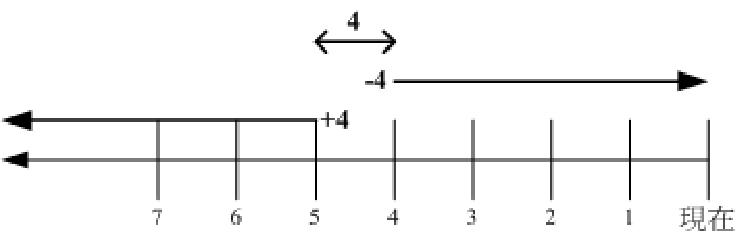
\includegraphics[scale=0.5]{pics/find_time}
		\item \op{user}: File is owned by user uname
		\item \op{group}: File belongs to group gname
		\item \op{perm}: File by permission. it support both symbolic(u+r) and number format(400). Just like time option, it also support n, -n and $\backslash$n(better format than +n). detail can be found in example.
		\item \op{path}: use when you want to exclude a directory	
		\end{itemize}
	\item[Actions in expression]:
		\begin{itemize}
		\item \op{print,print0,printf}: default actions is print
		\item \op{-exec }: execute some command
		\item \op{-prune}:
		\end{itemize}
	\item[Operators in expression]: \\
		\begin{tabular}{c|p{0.82\textwidth}}
		\hline
		() & Force  precedence \\
		! & no \\
		o & or \\
		, & both expr1 and expr2 are always evaluated \\
		\hline
		\end{tabular}
	\item[Example]:
		\begin{itemize}
		\item use of meta character \\
		\begin{tabular}{c|l}
		\hline \linuxcommand{find -name foo*bar} & shell will interpret * firstly(bad)\\
		\hline \linuxcommand{find -name foo$\backslash$*bar} & shell don't interpret *. \\
		\hline \linuxcommand{find -name ``foo*bar''} & the same as the previous  \\
		\hline \linuxcommand{find -name ``foo$\backslash$*bar''} & find exact file name. \\
		\hline
		\end{tabular}
		\item you also can use single quotes, but there is a different for shell
		\linuxcommand{find -name ``\$HOME''} will interpret it, but \linuxcommand{find -name '\$HOME'} will search it literaly. That's a very important difference bewteen them, you should know it.
		\item \linuxcommand{find /tmp /var/tmp . \$HOME -name foo 2>/dev/null} you can find in multi-directory and you can output error to /dev/null
		\item \linuxcommand{find / -mmin -10} learn which files got changed within 10 minnutes, it's also useful when you have download some file but can't locate it.(WATCH mmin, NOT mtime)
		\item \linuxcommand{find / -type f -mtime -7 | xargs tar -rf week\_add.tar} you can search files by two criteria. the default is \emph{and} relationship.
		\item \linuxcommand{find / -name /dev -prune | xargs tar \ldots} Normally, find returns the directory first, before any of the files in that directory.  This is useful when using the "-prune" action to prevent find from examining any files you want to ignore:
		\item \linuxcommand{find . -mmin +5 -mmin -10 } find files modifed between 6 and 9 minutes ago
		\item \linuxcommand{find . -maxdepth 1 -name '[!.]*' -printf 'Name: \%16f Size: \%6s$\backslash$n'} displays non-hidden (no leading dot) files in the current directory only (no subdirectories), with an custom output format:
		\item \linuxcommand{find . -type d | sort} get all directory and sort them.
		\item \linuxcommand{find /usr $\backslash$( -path /usr/sam1 -o -path /usr/sam2 $\backslash$) -prune -o -print} skip two directories when you conduct find.这个命令有点奇怪,我需要解释一下,prune通常只返回true,如果前面的path返回true,那么-o 后面的就没必要执行了,但是如果path返回false, 那么 path(false) and prune(true) 还是false.这个时候 -o后面的就得到执行的机会了。其实,find的各种应用形式,都是可以利用逻辑表达式的方式来理解的。当然,对于一些常用的应用,直接记住就可以了。
		\item \linuxcommand{find /    $\backslash$( -perm -4000 -fprintf /root/suid.txt '\%\#m \%u \%p$\backslash$n' $\backslash$) , $\backslash$ $\backslash$( -size +100M -fprintf /root/big.txt '\%-10s \%p$\backslash$n' $\backslash$)}  Traverse the filesystem just once, listing setuid files and directories into /root/suid.txt and large files into /root/big.txt.
		\end{itemize}
	\item[Note]:
		\begin{itemize}
		\item xargs is more efficent than -exec. 这是因为exec会把所有的参数传给后面的命令,如果参数过多,就会带来pararmter list is too long 这种错误。but it has two limitations. the first one is that not all commands accept the list of files at the end of the command, such as \linuxcommand{find -name $\backslash$*.txt | xargs cp /tmp} will not work. a solution is \linuxcommand{find -name $\backslash$*.txt | xargs -i cp \{\} /tmp}, to tell xargs use {} to replace the the result of find. Other solution is \linuxcommand{find -name $\backslash$*.txt | xargs cp -t /tmp}, and -t is an option scary for cp command. The other shortcoming is file name contain space. you can use \linuxcommand{find \ldots\ print0 | xargs -0 \ldots } to resolve this.
		\end{itemize}
	\end{description}
\section{grep}
	\linuxcommand{ grep [options] [-e PATTERN | -f FILE] [FILE...]}. you must specify files to search for, there is no default value. If it is empty, it will ask you to input something from standard input.
	\begin{description}
	\item[Options]: \\
		\begin{tabular}{c|p{0.82\textwidth}}
		\hline
		\op{i} & ignore case \\
		\op{v} & invert match\\
		\op{n} & show line name\\
		\op{w} & match the whole word, not substring \\
		\op{o} & only show match art, default show the match line\\
		\op{E} & support extend pattern\\
		\op{A, B, C} & after, before, context match.\\
		\hline
		\end{tabular}
	\item[PATTERN]:
		\begin{description}
		\item[Characters]: In fact, some grep don't support -P (perl options), you'd better avoid it. if you want to use ``* \^{} \$ [ ] \{ ( ) ? + '' literaly, you need to use $\backslash$ to escape it, or they have special meaning in the regular expression. dot stands for every character. if you want to match tab , you can use \hotkey{ctrl+v}, then tab to input a tab in a command line. below is common use characters.
		\begin{center}
			\begin{tabular}{|c|p{15em}|c|}
			\hline POSIX & Basic & perl \\
			\hline [[:alnum:]] & [0-9a-zA-Z] & $\backslash$w \\
			\hline [[:alpha:]] & [a-zA-Z] &  \\
			\hline [[:lower:]] & [a-z] &  \\
			\hline [[:upper:]] & [A-Z] &  \\
			\hline [[:digit:]] & [0-9] & $\backslash$d \\
			\hline [[:blank:]] & space and tab &  \\
			\hline [[:space:]] & more than blank, also include newline and carriage return &  \\
			\hline
			\end{tabular}
		\end{center}
	\item[Anchors]:
		\begin{itemize}
		\item \^{} begining of a line
		\item \op{\$} end of a line
		\item \op{$\backslash$< $\backslash$>}  begining of a word and end of a word. when you commit \linuxcommand{grep -E ``is$\backslash$>'' file} ``this's'' will be matched too.
		\end{itemize}
	\item[Alternations]:
		\begin{itemize}
		\item \op{|}: or, usually you put it within the a pair of ( ).
		\item \op{[]}: character set.
		\end{itemize}
	\item[Quantifiers]:
		\begin{itemize}
		\item \op{?} the preceding itme is optional and matched at most once
		\item \op{*} the preceding itme will be matched zero or moret times
		\item \op{+} the preceding itme will be matched one or moret times
		\item \op{\{n\}} the preceding itme will be matched exactly n times
		\item \op{\{n,\}} the preceding itme will be matched n or moret times
		\item \op{\{n,m\}} the preceding itme will be matched at least n times, but not moret than mtimes
		\end{itemize}
	\item[Grouping back references]:
		\begin{itemize}
		\item \op{()} group
		\item \op{$\backslash$num} back reference
		\end{itemize}
	\end{description}
	\item[Example]:
		\begin{itemize}
		\item \linuxcommand{grep -E ``love(rs|d)'' file} will match lovers and loved in file. you can't use [ ] to finish this task, because it only support single charater.
		\item \linuxcommand{grep -E ``$\backslash$([\^{}(]$\backslash$)''} to deal with this nest pairs, make sure that you can find the most inside
		\item \linuxcommand{grep ``EXIT\_'' /usr/include/*.h} You can search header files for particular definitions and
		function prototype.
		\item \linuxcommand{grep ``[]\^{} -]'' file} It's a little suprised, if you want to find ``] \^{} -'' you can put ]
		the first postion, put - the last postoin, and \^{}  everwhere but first position. in this way , you don't need escape them
		\item \linuxcommand{grep -c `date +\%b`} place a command inside a pair of backward marks
		\item \linuxcommand{grep 'a|b' file} doesn't work as your respect, you should use \linuxcommand{grep -E 'a|b' file}. you can see differences in Note.
		\end{itemize}
	\item[Note]:
		\begin{itemize}
		\item differences between grep and grep -E and egrep can be found in table ,
		you can concluded that best tool seem to be the \linuxcommand{grep -E} \\
		\begin{center}
 			\begin{tabular}{|c|c|c|}
			\hline grep & grep -E & egrep \\
			\hline $\backslash$+ & + or & yes \\
			\hline $\backslash$? & ? &  yes \\
			\hline ex1 $\backslash$| e2 & e1 | e2 & yes \\
			\hline $\backslash$(ex$\backslash$) & (ex) & yes \\
			\hline $\backslash${m,n$\backslash$} & {m,n} & no \\
			\hline no & $\backslash$w & $\backslash$w \\
			\hline no & $\backslash$< $\backslash$> & $\backslash$< $\backslash$> \\
			\hline
			\end{tabular}
		\end{center}
		\item Anyway, use -E is good habit. It can save your typing in the future.:)
		\end{itemize}
	\end{description}
\section{gzip}
	\begin{description}
	\item[Options]: \\
		\begin{tabular}{c|p{0.82\textwidth}}
		\hline
		\op{c} & output to screen, \\
		\op{d} & decompress \\
		\op{v} & verbose\\
		\op{r} & recursive directory, it will compress all files under this directory individually. \\
		\hline
		\end{tabular}
	\item[Example]:
		\begin{itemize}
		\item \linuxcommand{gzip -c file >file1.gz} By default, gzip will delete file and produce a file.gz. if you
		want to keep origanl one, you can use -c option like this example.
		\item \linuxcommand{gzip -d file1.gz}, it will produce file1 and delete file1.gz
		\end{itemize}
	\item[Note]:
		\begin{itemize}
		\item  by default, gzip will delete origal file, you don't need give it target file name.(it add .gz when compress or delete .gz when decompress
		\item \linuxcommand{zless} and \linuxcommand{zcat} to view the compress text file directly.
		\end{itemize}
	\end{description}
\section{bzip2}
	\begin{description}
	\item[Options]: \\
		\begin{tabular}{c|p{0.82\textwidth}}
		\hline
		\op{k} & keep original file, \\
		\op{1,\ldots 9} & level of compression. better compression, slower.\\
		\hline
		\end{tabular}
	\item[Example]:
		\begin{itemize}
		\item the options just like gzip, you can take a look at gzip command examples.
		\end{itemize}
	\item[Note]:
		\begin{itemize}
		\item  Compared with gzip, it don't support -r options, and other option is the same.
		\item \linuxcommand{bzless} and \linuxcommand{bzcat} to view the compress text file directly.
		\item In compression rate, the bzip2 is better than gzip. 文件名的后缀通常为bz2或者bz。如果是包文件,也可能是tbz2
		\end{itemize}
	\end{description}
\section{tar}
	\begin{description}
	\item[Options]:\\
		\begin{tabular}{c|p{0.82\textwidth}}
		\hline
		\op{p} & same permisstion \\
		\op{C} & extract to different directory \\
		\hline
		\end{tabular} \vspace{1ex} \\
		
		\begin{tabular}{|c|c|c|}
		\hline j(bzip2) & c(create) &   \\ \cline{2-2}
			& t(check) & v(verbose) \\ \cline{2-2}
			z(gzip)  & x(extract) &   \\
		\hline
		\end{tabular}
	\item[Example]:
		\begin{itemize}
		\item \linuxcommand{tar -xv -f file.tar} to extract file for tar ball
		\item \linuxcommand{tar -cv -f file.tar dirName} to create a tar ball contain the whole dirName
		\item \linuxcommand{tar -jxv -f file.tbz2 -C /tmp} to extract and unzip a tar ball and copy it the /tmp
		\end{itemize}
	\item[Note]:
		\begin{itemize}
		\item  You'd better use -f to specify tar.gz name seperately. It's more obvious.
		\end{itemize}
	\end{description}
\section{file}
	\begin{description}
	\item[Options]: \\
		\begin{tabular}{c|p{0.82\textwidth}}
		\hline
		\op{s} & read special file \\
		\hline
		\end{tabular}
	\item[Example]:
		\begin{itemize}
		\item \linuxcommand{sudo file -s /dev/hda1} you can use -s optoin, and you also need root permission.
		\end{itemize}
	\item[Note]:
		\begin{itemize}
		\item  usually, file name doesn't have extension, use file to know what type it is. linux系统文件通常没有后缀名,所以你最好用file命令先判断一下这个文件是个什么类型的文件。
		\end{itemize}
	\end{description}
\section{locate}
	\begin{description}
	\item[Options]: \\
		\begin{tabular}{c|p{0.82\textwidth}}
		\hline
		\op{w} & default, whole name\\
		\op{b} & Results are considered to match if the pattern specified matches the final component of the name of a file as listed  in the database.  This final component is usually referred to as the `base name'. \\
		\hline
		\end{tabular}
		
	\item[Example]:
		\begin{itemize}
		\item \linuxcommand{locate linux.tex} will output linux.tex and linux.tex.backup
		\item \linuxcommand{locate -b ``$\backslash$linux.tex''} will only output linux.tex
		\end{itemize}
	\item[Note]:
		\begin{itemize}
		\item  locate search file in a database file. \linuxcommand{updatedb} to update this database
		\end{itemize}
	\end{description}
\section{which}
	\begin{description}
	\item[Options]: \\
		\begin{tabular}{c|p{0.82\textwidth}}
		\hline
		 \op{a} & print all matching pathname\\
		\hline
		\end{tabular}
	\item[Example]:
		\begin{itemize}
		\item \linuxcommand{which ls}
		\end{itemize}
	\item[Note]:
		\begin{itemize}
		\item  only located command, you can use \linuxcommand{find} for ordinary file.
		\end{itemize}
	\end{description}
\section{whereis}
	locate binary, source and manual of file(command)
	\begin{description}
	\item[Options]:\\
		\begin{tabular}{c|p{0.82\textwidth}}
		\hline
		 \op{empty} & empty\\
		\hline
		\end{tabular}
	\item[Example]:
		\begin{itemize}
		\item \linuxcommand{whereis man} output is
		\begin{screen}
		/usr/bin/man /usr/local/man /usr/share/man /usr/share/man/man1/man.1.gz  /usr/share/man/man7/man.7.gz
		\end{screen}
		there are two different kind of manual page for man, you can use \linuxcommand{man 1 man} and \linuxcommand{man 7 man } to read them. Meanings of number can be found in man 1 man.
		\end{itemize}
	\item[Note]:
		\begin{itemize}
		\item  it seems that it commonly used for command and not for ordinary file, just like which.
		\end{itemize}
	\end{description}
\section{ps}
	process status report a snapshot of the current processes
	\begin{description}
	\item[Options]: \\
		\begin{tabular}{c|p{0.82\textwidth}}
		\hline
		 \op{a} & select all process except session leader(?)\\
		\hline
		\end{tabular}
	\item[Example]:
		\begin{itemize}
		\item \linuxcommand{ps -ux} list current user process
		\item \linuxcommand{ps -aux | grep 'name' }
		\end{itemize}
	\item[Note]:
		\begin{itemize}
		\item  you can find STAT code in by \linuxcommand{man ps}
		\end{itemize}
	\end{description}
\section{kill}
	send a singal to a process
	\begin{description}
	\item[Options]: \\
		\begin{tabular}{c|p{0.82\textwidth}}
		\hline
		\op{l} & list all aviable singal.\\
		\hline
		\end{tabular}
		
	\item[Example]:
		\begin{itemize}
		\item \linuxcommand{kill -9 -1} kill all processes you can kill
		\item \linuxcommand{kill 123} send SIGTERM to pid 123,
		\end{itemize}
	\item[Note]:
		\begin{itemize}
		\item  you should use \linuxcommand{ps} to find pid value.
		\item  -9 means kill, This will not be blocked by the application.
		\end{itemize}
	\end{description}
\section{jobs}
	list the jobs you are runing in the backgroud and foreground
	\begin{description}
	\item[Options]:\\
		\begin{tabular}{c|p{0.82\textwidth}}
		\hline
		 \op{empty} & empty\\
		\hline
		\end{tabular}
	\item[Example]:
		\begin{itemize}
		\item
		\end{itemize}
	\item[Note]:
		\begin{itemize}
		\item it will output job num,usually use before \linuxcommand{fg jobnum}and \linuxcommand{ bg jobnum}to
		\item you can ues \linuxcommand{command \&} to put it to background \emph{running}, When you use Ctrl+Z,
		it just put the current processing to background \emph{suspending}, then you can use bg to change it to
		background \emph{running}. \linuxcommand{fg jobnum} can put it ot foreground running, at this time, you
		can use Ctrl+C to stop it. Or use kill in other terminal console.
		\end{itemize}
	\end{description}
\section{wc}
	word count, print line, word, and byte count of a file
	\begin{description}
	\item[Options]: \\
		\begin{tabular}{c|p{0.82\textwidth}}
		\hline
		\op{l} & only print line number \\
		\op{w} & only print word number\\
		\op{m} & only print character number\\
		\op{L} & print the longest line\\
		\hline
		\end{tabular}
	\item[Example]:
		\begin{itemize}
		\item \linuxcommand{wc -l file}
		\end{itemize}
	\item[Note]:
		\begin{itemize}
		\item  \op{L} is very interesting option
		\end{itemize}
	\end{description}	

\section{history}
	list all commands you have typed.
	\begin{description}
	\item[Options]: \\
		\begin{tabular}{c|p{0.82\textwidth}}
		\hline
		\hline
		\end{tabular}
	\item[Example]:
		\begin{itemize}
		\item \linuxcommand{history | grep command1} to search a command in a long history list.
		\end{itemize}
	\item[Note]:
		\begin{itemize}
		\item
		\end{itemize}
	\end{description}	

\section{lp}
	print a document
	\begin{description}
	\item[Options]: \\
		\begin{tabular*}{0.9\textwidth}{c|l}
		\hline
		\op{sides=two-sided-long-edge} & two sides print\\
		\hline
		\end{tabular*}
	\item[Example]:
		\begin{itemize}
		\item \linuxcommand{fmt a.txt |pr| lp} fmt is simple command, just create a longer praragraph. And pr maybe can add page number to the page
		\end{itemize}
	\item[Note]:
		\begin{itemize}
		\item  It seems that lp is better than lpr because it is more compatiable.
		\end{itemize}
	\end{description}
\section{sort}
	sort lines of text file
	\begin{description}
	\item[Options]:\\
		\begin{tabular}{c|p{0.82\textwidth}}
		\hline
		\op{f} & make all lines uppercase before sorting \\
		\op{d} & --dictionary-order\\
		\op{f} & --ignore-case\\
		\op{n} & --numeric-sort\\
		\op{r} & --reverse the result of comparisons\\
		\op{+m} & start at the first character of m+1th fiedl\\
		\op{-n} & end at the last character of the nth field\\
		\op{tx} & use x as the field delimiter\\
		\hline
		\end{tabular}
	\item[Example]:
		\begin{itemize}
		\item \linuxcommand{sort -r +2 -3 company.data}
		\item \linuxcommand{sort -t: +1 -2 company.data}
		\end{itemize}
	\item[Note]:
		\begin{itemize}
		\item It's often used in pipe
		\item You also can sort according to two columns
		\end{itemize}
	\end{description}
\section{less}
	\begin{description}
	\item[Options]: \\
		\begin{tabular}{c|p{0.82\textwidth}}
		\hline
		\op{N} & print line number \\
		\hline
		\end{tabular}
	\item[Example]:
		\begin{itemize}
		\item \linuxcommand{file1 file2 file3} you can use :n :q to navigate these files
		\item you can use v command to open your default editor in less
		\item :e to open a new document, :d to delete the current one
		\end{itemize}
	\item[Note]:
		\begin{itemize}
		\item It's more like only read editor, you should use different commands to control it.
		\item if you forget some commands usage, you can use command h .
		\end{itemize}
	\end{description}
\section{uniq}
	report or omit repeated lines
	\begin{description}
	\item[Options]: \\
		\begin{tabular}{c|p{0.82\textwidth}}
		\hline
		\op{c} & prefix lines by the number of occurrences \\
		\hline
		\end{tabular}
	\item[Example]:
		\begin{itemize}
		\item \linuxcommand{sort file | uniq -c } give you unigram information
		\end{itemize}
	\item[Note]:
		\begin{itemize}
		\item It must be used in a sorted file
		\end{itemize}
	\end{description}
\section{xxd}
	make a hexdump or do the reverse
	\begin{description}
	\item[Options]:\\
		\begin{tabular}{c|p{0.82\textwidth}}
		\hline
		\op{b} & switch to bits(binary digits) dump \\
		\op{c cols} & format cols octets per line\\
		\op{l len} & stop after writing len octets\\
		\hline
		\end{tabular}
	\item[Example]:
		\begin{itemize}
		\item \linuxcommand{xxd -l 120 -c 12 xxd.1}
		\end{itemize}
	\item[Note]:
		\begin{itemize}
		\item a similar command is like \linuxcommand{od -t x1}, default output of od
		is based on octal, the output is little strange, because it divived binary bit every three bits, for exmaple 00100000 00100000 od -t o1 will outupt 040 040, and od -t o2 will output 020040 (0,010,000,0 00,100,000). Do you still understand it:)
		\end{itemize}
	\end{description}
\section{cut}
	remove sections from each line of a file
	\begin{description}
	\item[Options]: \\
		\begin{tabular}{c|p{0.82\textwidth}}
		\hline
		\op{d} & field delimiter \\
		\op{f} & for field \\
		\op{c} & field delimiter is character\\
		\hline
		\end{tabular}
	\item[Example]:
		\begin{itemize}
		\item \linuxcommand{cut -d``*'' -f 2-3} will output B*C. it will not change the original content, only cut part of out
		\end{itemize}
	\item[Note]:
		\begin{itemize}
		\item If you need change format from the inputfile, \linuxcommand{awk} or \linuxcommand{sed } is two better choices.
		\end{itemize}
	\end{description}
\section{type}
	\linuxcommand{type }: Using the "type" command shows how any of the commands or names you include beyond the command would be interpreted if input. This means that it would explain any macros you created, any commands you've aliased or any other additions you've made to the BASH
	\begin{description}
	\item[Options]: \\
		\begin{tabular}{c|p{0.82\textwidth}}
		\hline
		\op{a} Using "-a" will display a list of all executables with the file name.
		\op{t} Using "-t" will display a single word relating to the actual type of the command you wish to describe (alias, function, builtin, keyword or file).
		\op{p} Using "-p" will display the name of the file used with the "type" command.
		\end{tabular}
	\item[Example]:
		\begin{itemize}
		\item empty
		\end{itemize}
	\item[Note]:
		\begin{itemize}
		\item it's a little like \linuxcommand{whereis}
		\end{itemize}
	\end{description}

\section{tr}
	translate or delete characters
	\linuxcommand{tr [option] \ldots SET1 [SET2]}
	\begin{description}
	\item[Options]: \\
		\begin{tabular}{c|p{0.82\textwidth}}
		\hline
		\op{c} & --complement \\
		\op{d} & --delete\\
		\op{s} & --squeeze-repeats\\
		\op{t} & --truncate-set1, may be used only when translating.
		Interpreted sequences are $\backslash$NNN, $\backslash$b backspace, $\backslash$n new line $\backslash$r return, $\backslash$t horizontal tab, $\backslash$v vertical tab. It also can contain [:alnum:] [:digit:] \\
		\hline
		\end{tabular}
	\item[Example]:
		\begin{itemize}
		\item \linuxcommand{tr A-z a-z <a.txt | tr -d ``.,?''|tr -s ' ' '$\backslash$012'|sort|unqi -c} this command will
		produce a unigram for a text file.
		\end{itemize}
	\item[Note]:
		\begin{itemize}
		\item It mainly applied in character level.
		\item It doesn't include file name argument, you should use <file.name to redirect.
		\end{itemize}
	\end{description}
\section{join}
	join lines of two files on a common field
	\begin{description}
	\item[Options]: \\
		\begin{tabular}{c|p{0.82\textwidth}}
		\hline
		\op{t} & delimiter character \\
		\op{i} & ignore case \\
		\op{1 num} & use this num to specify field in the first file \\
		\op{2 num} & use this num to specify field in the second file \\
		\hline
		\end{tabular}		
	\item[Example]:
		\begin{itemize}
		\item
		\begin{screen}
		==> /etc/passwd <==  \\
		root:x:0:0:root:/root:/bin/bash \\
		bin:x:1:1:bin:/bin:/sbin/nologin \\
		daemon:x:2:2:daemon:/sbin:/sbin/nologin \\

		==> /etc/group <== \\
		root:x:0:root \\
		bin:x:1:root,bin,daemon \\
		daemon:x:2:root,bin,daemon \\
		\end{screen}
		
		\linuxcommand{join -t ':' -1 4 /etc/passwd -2 3 /etc/group}
		will produce output like this \\

		\begin{screen}
		0:root:x:0:root:/root:/bin/bash:\textit{root:x:root} \\
		 1:bin:x:1:bin:/bin:/sbin/nologin:\textit{bin:x:root,bin,daemon} \\
		 2:daemon:x:2:daemon:/sbin:/sbin/nologin:\textit{daemon:x:root,bin,daemon} \\
		\end{screen}
		\end{itemize}
	\item[Note]:
		\begin{itemize}
		\item
		\end{itemize}
	\end{description}
\section{du}
	estimate file space usage
	\linuxcommand{tr [option] \ldots SET1 [SET2]}
	\begin{description}
	\item[Options]: \\
		\begin{tabular}{c|p{0.82\textwidth}}
		\hline
		\op{c} & --total, produce a grand total \\
		\op{h} & --human-readable\\
		\op{s} & --summarize, display only a total for each argument\\
		\hline
		\end{tabular}	
	\item[Example]:
		\begin{itemize}
		\item \linuxcommand{du -sch *} this command will
		print all directory size
		\item \linuxcommand{du -sh *} will print all leaf directory
		size
		\end{itemize}
	\item[Note]:
		\begin{itemize}
		\item you must give a directory name or * as a argument.
		\end{itemize}
	\end{description}
\section{dos2unix}
	Converts text files between DOS and Unix formats.
	\begin{description}
	\item[Options]: \\
		\begin{tabular}{c|p{0.82\textwidth}}
		\hline
		\op{empty} & empty \\
		\hline
		\end{tabular}
	\item[Example]:
		\begin{itemize}
		\item \linuxcommand{dos2unix file} this command will change return format.
		\end{itemize}
	\item[Note]:
		\begin{itemize}
		\item \linuxcommand{unix2dos} does the reverse thing
		\item it will overwrite the input file directly
		\end{itemize}
	\end{description}
\section{tail}
	output the last part of files
	\begin{description}
	\item[Options]: \\
		\begin{tabular}{c|p{0.82\textwidth}}
		\hline
		\op{n} & --lines=N output the last N lines, instead of the last 10 \\
		\op{f} & --follow, output appended data as the file grows \\
		\hline
		\end{tabular}
	\item[Example]:
		\begin{itemize}
		\item \linuxcommand{tail -f log} this command will monitor the log file
		\end{itemize}
	\item[Note]:
		\begin{itemize}
		\item empty
		\end{itemize}
	\end{description}
\section{ldd}
	print shared library dependencies
	\begin{description}
	\item[Options]: \\
		\begin{tabular}{c|p{0.82\textwidth}}
		\hline
		\op{empty} & empty \\
		\hline
		\end{tabular}
	\item[Example]:
		\begin{itemize}
		\item \linuxcommand{ldd $\backslash$bin$\backslash$ls}
		\end{itemize}
	\item[Note]:
		\begin{itemize}
		\item empty
		\end{itemize}
	\end{description}
\section{lpq}
	show printer queue status
	\begin{description}
	\item[Options]: \\
		\begin{tabular}{c|p{0.82\textwidth}}
		\hline
		\op{empty} & empty \\
		\hline
		\end{tabular}
	\item[Example]:
		\begin{itemize}
		\item \linuxcommand{lpq}
		\end{itemize}
	\item[Note]:
		\begin{itemize}
		\item \linuxcommand{lprm} to delete a print task
		\item \linuxcommand{lp} to print a document
		\end{itemize}
	\end{description}
\section{free}
	Display amount of free and used memeory in the sytem
	\begin{description}
	\item[Options]: \\
		\begin{tabular}{c|p{0.82\textwidth}}
		\hline
		\op{b} & dispaly in byte, and you can think there are other options, k,m,g \\
		\hline
		\end{tabular}
	\item[Example]:
		\begin{itemize}
		\item \linuxcommand{free -m}
		\end{itemize}
	\item[Note]:
		\begin{itemize}
		\item
		\end{itemize}
	\end{description}
\section{netstat}
	Print network connections, routing tables.
	\begin{description}
	\item[Options]: \\
		\begin{tabular}{c|p{0.82\textwidth}}
		\hline
		\op{empty} & empty\\
		\hline
		\end{tabular}
	\item[Example]:
		\begin{itemize}
		\item \linuxcommand{netstat -m}
		\end{itemize}
	\item[Note]:
		\begin{itemize}
		\item \op{a} and \op{n} are used more often.
		\end{itemize}
	\end{description}
\section{nl}
	number lines of files
	\begin{description}
	\item[Options]: \\
		\begin{tabular}{c|p{0.82\textwidth}}
		\hline
		\op{empty} & empty\\
		\hline
		\end{tabular}
	\item[Example]:
		\begin{itemize}
		\item
		\end{itemize}
	\item[Note]:
		\begin{itemize}
		\item  you can use less -N to get the same result, but here, it support some logical page which inlcudes header, body and footer
			The beginnings of the sections of logical pages are indicated in the input file by a line containing nothing except one of the following delimiter strings:
			$\backslash$:$\backslash$:$\backslash$: start of header \\
			$\backslash$:$\backslash$: start of body \\
			$\backslash$: start of footer \\
		\end{itemize}
	\end{description}
\section{diff}
	Display amount of free and used memeory in the sytem
	\begin{description}
	\item[Options]:\\
		\begin{tabular*}{0.9\textwidth}{c|l}
		\hline
		\op{y} & Display two columns \\
		\op{--suppress-common-lines} & Do not output common lines \\
		\hline
		\end{tabular*}
	\item[Example]:
		\begin{itemize}
		\item
		\end{itemize}
	\item[Note]:
		\begin{itemize}
		\item \linuxcommand{diff new.log old.log | grep \^{} $\backslash$< | wc -l} find how  many difference.
		\end{itemize}
	\end{description}	
\section{df}
	report filesystem disk space usage
	\begin{description}
	\item[Options]: \\
		\begin{tabular}{c|p{0.82\textwidth}}
		\hline
		\op{h} & dispaly human-readable\\
		\hline
		\end{tabular}
	\item[Example]:
		\begin{itemize}
		\item \linuxcommand{df -h}
		\end{itemize}
	\item[Note]:
		\begin{itemize}
		\item It is a little different with du, and du is used more often.
		\end{itemize}
	\end{description}
\section{pdftops}
	pdftops - Portable Document Format (PDF) to PostScript converter (version 3.00)
	\begin{description}
	\item[Options]:\\
		\begin{tabular}{c|p{0.82\textwidth}}
		\hline
		\op{eps} & produce eps picture\\
		\hline
		\end{tabular}
	\item[Example]:
		\begin{itemize}
		\item \linuxcommand{pdftops -eps file.pdf file.eps}
		\end{itemize}
	\item[Note]:
		\begin{itemize}
		\item First, you can use printer to print visio to pdf, than use this command to change
		it to eps, and \LaTeX\ support eps. that is good.
		\end{itemize}
	\end{description}
\section{wget}
	non-interactive network downloader.
	\begin{description}
	\item[Options]:\\
		\begin{tabular}{c|p{0.82\textwidth}}
		\hline
		\op{empty} & empty \\
		\hline
		\end{tabular}
	\item[Example]:
		\begin{itemize}
		\item \linuxcommand{wget -r -np -nd --accept=iso http://example.com/i386/} 其中,-np 的作用是不遍历父目录,-nd 表示不在本机重新创建目录结构。--accept=iso 选项,这指示 wget 仅下载 i386 目录中所有扩展名为 iso 的文件。你也可以指定多个扩展名,只需用逗号分隔即可。
		\end{itemize}
	\item[Note]:
		\begin{itemize}
		\item
		\end{itemize}
	\end{description}

\chapter{Application}
\section{Ubuntu}
		\begin{itemize}
		\item 取消屏幕锁定,系统--首选项--屏幕保护程序。
		\item Nautilus start typing the search term. A small search text field will appear near the bottom-right of the window and files/folders will be matched as you type
		\item unrar  filename.rar, replacing filename.rar with that which you downloaded
		\item Click System ->Administration-> Software Sources. Click the Download from dropdown list and then select Other. In the list of servers, choose any you wish. You'll need to reload the package lists from the server when prompted.
		\item If Windows didn't cleanly shutdown then Ubuntu will refuse to mount the partition. If, even after Windows is cleanly shutdown, the Windows partition refuses to appear, then run a chkdsk on the partition from within Windows.
		\item Terminal click Edit -> Current Profile and select the Colors tab. Then remove the check from Use colors from system theme and select a replacement from the Built-in schemes dropdown list. Try the Green on Black scheme.
		\item Alt + F2 . Then type the name of the program. If it needs to run with root privileges, just type gksu beforehand.
		\item If Windows is refusing to boot, for whatever reason, you can try repairingthe file system from within Ubuntu. Use Synaptic to search for the ntfsprogs package. Once it's installed, unmount your Windows partition (if it's mounted) and
		type sudo ntfsfix /dev/sda1 to check and fix the partition (assuming your Windows partition is /dev/sda1. likely if you installed Ubuntu in a dual-boot configuration on a computer already running Windows).
		\item The following will send everything currently on the current screen (command-line prompts included) to a text file called output.txt:\$ sudo screendump > output.txt
		The command has to be issued as root because of permission issues but the resulting file will be owned by you.
		\item 	If you're working on a virtual console and want to kill the GUI for any reason, typing the following will kill GNOME Display Manager (gdm), which ``owns'' the desktop processes:
		\linuxcommand{sudo killall gdm}. To get the GUI back following this, start gdm again: \linuxcommand{sudo gdm}
		\item do the following:open a terminal window and type \linuxcommand{cat /etc/lsb-release}. You can also click Help ! About Ubuntu to check version
		\item click System->Preferences->Keyboard Shortcuts and look in the list for Run a Terminal, which will be under the Desktop heading. Click the word Disabled alongside it, and then hit Ctrl + Alt + t .
		\item Start Firefox and, in the address line, type about:plugins. The headings show the type of content the plugin is designed to pick-up and below is listed the Ubuntu plugin that handles the content.
		\item To check virus, To install ClamTK and also ClamAV, use Synaptic to search for the clamtk package.
		\item To quickly view a picture from the command line, just type \linuxcommand{eog filename}.
		\item To move any unmaximized window around, hold down Alt and then click and drag anywhere in the window.
		\item There are a number of ways of converting a text file into a PDF at the command line. Perhaps easiest is to ``print'' it to Ubuntu's PDF printer driver. The file will then be saved to the PDF folder in your /home folder. This tip uses the lp command, telling it which printer to use with the options \op{d} : \linuxcommand{lp -d PDF textfile.txt}
		\item Uninstall Ubuntu can be seen in ubuntu\_kung\_fu tip 118
		\item \linuxcommand{sudo mkdir /media/ISO }, \linuxcommand{sudo mount -o loop ~/ubuntu.iso /media/ISO}
		Note that the first command creates a mount point and doesn't need to be typed in future. Once the ISO image is mounted, an icon for it will automatically appear on the desktop.To unmount the image, type sudo umount /media/ISO in the terminal window.
		\item To clear the cache from the command-line, type the following: \linuxcommand{sudo apt-get clean}
		\item use the pdftotext program: pdftotext filename.pdf. This will create a .txt file containing the contents of the PDF. To view it, use the less command: less filename.txt. To extract the images from the PDF, use the pdfimages command. You'll need to specify the filenames for the pictures, and also the -j command option to ensure the photographic images are outputted as JPEG. For example, the following: \linuxcommand{pdfimages -j filename-pdf pictures}
		\item Start your favorite application, highlight the mouse cursor over the menu option you want to change, and hit the new
		combination. You'll see that the menu instantly reflects the changes. To remove any keyboard shortcut, just hit the Backspace key
		(not the Delete key?that will cause Delete to be the new shortcut).
		\item Just use Synaptic to install nautilus-open-terminal. Then log out and back in again. In future you can either right-click blank
		space in a particular folder and select Open in terminal to open a terminal window automatically in that folder
		% \item Now run it through the column command by piping the output of the previous command, as follows: \$ cat /etc/fstab|column ?t
		\item \$ xclip < /etc/fstab
		...which will add the contents of the /etc/fstab configuration file to the clipboard, or you can pipe the output of a command into it:
		\linuxcommand{dmesg|xclip}
		...which will place the output of the dmesg command in the clipboard (dmesg shows system log output, and can be useful when diagnosing problems).
	\end{itemize}

\section{KDE}
		\begin{itemize}
		\item Konqueror F9 will show or hide Navigation Panel! F4 will open shell window. I mainly use mc now.
		\item in Konsole, you can press shift+-> to jump to another Shell window, it's convenient for you to finish some tasks
		\end{itemize}

\ifx \allfiles \undefined
\end{CJK*}
\end{document}
\fi	
